%
% File: chap01.tex
% Author: Solal Rapaport
% Description: Introduction chapter.
%
\let\textcircled=\pgftextcircled
\chapter{Introduction}
\label{chap:intro}

\initial{C}ats are beautiful. \lipsum[12]
\TODO{Write a real introduction.}

I love cats. \lipsum[1]

%=======
\section{Section}
\label{sec:sec01}

Dogs~\footnote{american shepherd mostly}
\TODOside{Add proper references}
are also very beautiful~\cite{tmp}.

\subsection{Subsection}
\label{subsec:subsec01}

Let's deep-dive into cats.

%A figures matrix.
\begin{figure}[t!]
\centering
\begin{minipage}{3.3cm}
    \centering
    \subtop[]{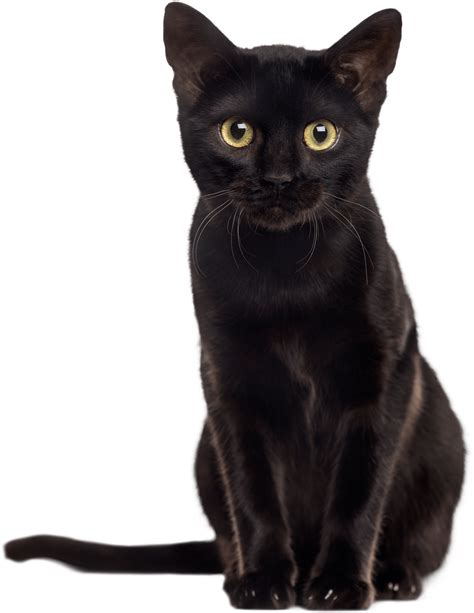
\includegraphics[height=0.28\textheight]{fig01/black}\label{cat1}}
\end{minipage}
\hspace{0.5cm}
\begin{minipage}{3.3cm}
    \centering
    \subtop[]{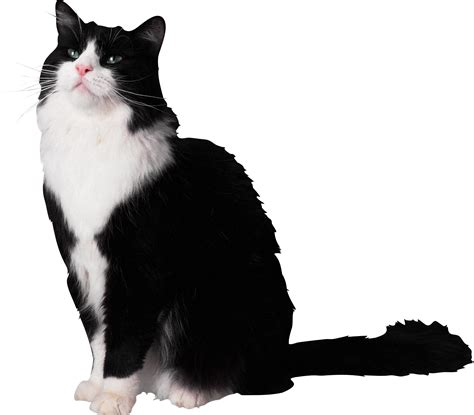
\includegraphics[height=0.27\textheight]{fig01/suit}\label{cat2}}
\end{minipage}
\hspace{1.3cm}
\begin{minipage}{3.3cm}
    \centering
    \subtop[]{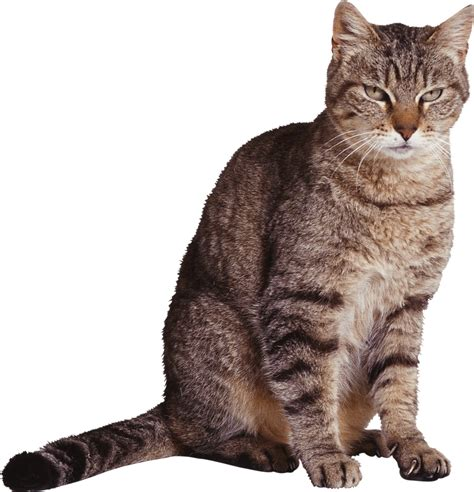
\includegraphics[height=0.27\textheight]{fig01/suspicious}\label{cat3}}
\end{minipage}
\\ \vspace{0.1cm}
\begin{minipage}{10cm}
    \centering
    \subtop[]{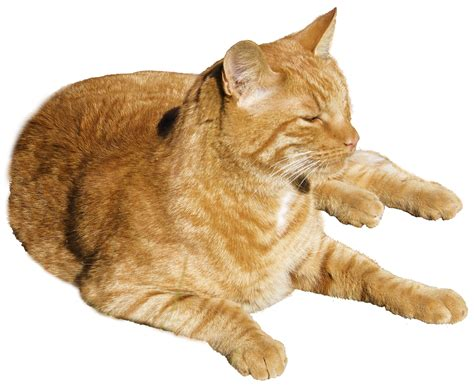
\includegraphics[height=0.145\textheight]{fig01/orange}\label{cat4}}
\end{minipage}
\\ \vspace{0.1cm}
\begin{minipage}{10cm}
    \centering
    \subtop[]{
\includegraphics[height=0.16\textheight]{fig01/white}\label{cat5}}
\end{minipage}
\mycaption[Single cats.]{(a) A black cat. (b) A suit cat. (c) A suspicious cat. (d) An orange cat. (e)~A white cat.}
\label{fig:singlecat}
\end{figure}

% A single figure
\begin{figure}[t!]
	\centering
	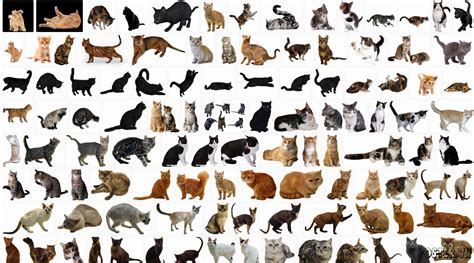
\includegraphics[height=0.35\textheight]{fig01/cats}
	\mycaption[All cats.]{A lot of cats.}
	\label{cats}
\end{figure}

%=========================================================